\section{Intelligence as a Service}

\paragraph{} Il est important en premier lieu de comprendre comment est né le terme d'intelligence
artificielle et ce qu'il implique techniquement. L'IA est un domaine de l'informatique et se définit
comme l'étude des \emph{agents intelligents} : c'est-à-dire tout appareil en mesure de perçevoir son
environnement, et de prendre les actions en conséquence afin de maximiser ses chances de succès pour
le même objectif donné. \cite{AI0} Elle s'applique également aux fonctions cognitives qui
imitent l'humain, à l'exemple de \emph{l'apprentissage} ou de la \emph{résolution de problèmes}.

\paragraph{} Néanmoins, l'intelligence artificielle n'a pas toujours eu le même sens, ni comporté
tous les domaines présents aujourd'hui. Pour certains, elle désignerait uniquement ce qui n'a
pas encore été réalisé, comme la création d'une machine dotée d'une intelligence humaine et autonome.
On peut comprendre en ce sens que l'IA s'attache à essayer de conçevoir et de comprendre des faits
dans des domaines vastes et en perpétuelle évolution. Nous verrons par la suite que, même si
l'utilisation d'intelligences s'est \emph{démultipliée} de manière \emph{exponentielle} ces vingt
à soixante dernières années, le terme est encore utilisé parfois à tort ou de manière imprécise 
pour désigner des concepts mal compris. Cela s'explique notamment par l'utilisation abusive du terme 
par les médias, qui en font \emph{un buzzword}, et \emph{désinforment parfois} l'auditeur.
Par ailleurs, nous avons vu que la littérature et la science-fiction en particulier envisagent des
scénarii qui ne se révèlent pas nécessairement exacts. 

\paragraph{Objet d'étude} Les domaines d'études usuels de la recherche en intelligence artificielle sont le
\emph{raisonnement}, la \emph{perception}, l'\emph{apprentissage}, la \emph{connaissance}, la
\emph{prévision}, le \emph{traitement du langage naturel} (ou TLN, Natural Language Processing en anglais),
et en robotique l'habileté de \emph{se déplacer}, ou encore de \emph{déplacer} ou \emph{manipuler} des
objets. Son application nécessite l'utilisation d'outils comme l'\emph{optimisation}, la \emph{théorie des graphes},
mais aussi des méthodes statistiques et des notions de probabilité. 

\paragraph{Turing, adaptabilité, approches symbolique et connexionniste}

\paragraph{} Historiquement, c'est au milieu des années 50 qu'apparaît le termne d'intelligence artificielle, que l'on
doit à John McCarthy, aussi connu pour être le \emph{père de l'intelligence artificielle}. \cite{AI2} C'est également
dans les mêmes années qu'Alan Turing réalise un essai bien connu, \emph{The Imitation Game} (ou jeu d'imitation), procédé
permettant de déterminer si une machine est intelligente ou non. Pour cela, dans sa dernière version, le test de turing
propose à un être humain, placé dans une salle, de discuter avec deux personnes : une réelle, une autre simulée par une
machine. Si le sujet n'arrive pas à reconnaître quelle personne est réelle dans plus de la moitié des cas, alors on
considère que la machine à passé le test de Turing. \cite{Turing0}

\paragraph{} Ce test subit, à l'instar du test de QI, de nombreuses critiques. Il ne s'applique pas, en effet, à toutes
les formes d'intelligence mais uniquement aux programmes destinés à la communication. De plus, un programme \guillemotleft
non intelligent\guillemotright, c'est-à-dire conçu pour ruser le test, peut très bien le faire à l'exemple d'ELIZA.
\cite{Language0} Il utilise pour cela des mots de phrases précédentes qu'il réutilise pour poser des questions. Ce logiciel
se retrouve aussi comme psychologue dans l'éditeur de texte Emacs. \cite{Therapy0} Il est également intéressant de constater
que les logiciels \emph{trop intelligents} ne fonctionnent pas : en ne faisant jamais de fautes et en pratiquant une grammaire
et des tournures parfaites, le sujet se doute rapidement que son interlocuteur n'est pas humain.

\paragraph{} L'intelligence artificielle est donc une recherche \emph{d'adaptabilité}. Elle cherche à mettre en place des
stratégies \emph{souples}, qui répondent \emph{au mieux dans la plupart des cas}. On peut, dans ce grand courant, découper
deux types d'approches en particulier :
\begin{itemize}
    \item Symbolique : l'environnement et les lois qui s'y appliquent sont décrites avec le plus de précision possible,
    et il attendu du programme de choisir la meilleure option. C'est le cas par exemple des systèmes experts ou des
    logiques floues. Cette approche nous intéresse moins que la seconde car elle demande que les systèmes soient \emph{
    explicites}, et s'adapte donc mal à des cas \emph{réels}.
    \item Connexionniste : seul est donné au logiciel le moyen d'évaluer si ce qu'il fait est bien ou non - on le laisse
    en effet trouver des solutions \emph{seul, par émergence}. Les réseaux de neurones font partie de cette catégorie.
\end{itemize}

\paragraph{Utilisation de l'IA dans différents domaines}

\paragraph{} L'intelligence artificielle, nous la connaissons souvent le mieux associée avec la science-fiction. On
la vit parfois dangereusement, comme l'ordinateur HAL 9000 de l'Odyssée de l'Espace de Stanley Kubrick \cite{Kubrick0},
qui se rebelle contre les astronautes du vaisseau qu'il dirige. Asimov lui établit le code des robots dans son oeuvre
Le Cycle des Robots. \emph{Asimov1} Et l'IA est effectivement utilisée dans le monde de \emph{la robotique} pour permettre aux
robots d'intéragir de manière \emph{plus souple avec les humains qu'ils doivent aider}. \cite{AI1} Les tâches de ces 
robots peuvent être simples comme laver mais également bien plus complexe lorsqu'il s'agit par exemple d'aider une
personne n'ayant plus toutes ses capacités - une personne âgée ou en situation de handicap. Le domaine \emph{militaire} utilise
d'ailleurs l'IA à travers notamment de la robotique, avec l'utilisation de drones, la création de soldats mécaniques,
mais aussi des robots qui permettraient de localiser et sauver des victimes de catastrophes naturelles.

\paragraph{} Un autre grand domaine d'application de l'intelligence artificielle est le \emph{jeu vidéo}. L'utilisation 
d'automates et de chemins prédéfinis, comme les ennemis dans Mario par exemple, ne suffisent pas à permettre la réalisation
de jeux \emph{réalistes} dans certains domaines. On attend par exemple, dans un jeu de rôle ou un jeu d'aventure, que les
personnages aient un comportement qui paraisse le plus cohérent possible. Même des jeux très simples en terme de contenu
comme PacMan possèdent une part d'IA : chaque fantôme à un objectif différent.

\paragraph{} Et si la robotique et le jeu vidéo semblent des domaines d'application évidents, l'IA s'applique également
à bien d'autres domaines. Dans le milieu \emph{bancaire}, elle permet de détecter des fraudes à la carte bancaire. En
\emph{médecine}, certaines machines peuvent proposer des diagnostics en fonction des symptômes du patient, et ce de
manière plus rapide et complète qu'un médecin, même si ce dernier reste \emph{indispensable pour la prise de décision}.
En \emph{informatique industrielle} l'IA est utilisée en logistique, pour optimiser les trajets des transporteurs ou 
encore le remplissage de ces derniers. Le rangement d'un entrepôt peut également être optimisé grâce à des algorithme d'IA.
Les composants fabriqués peuvent être rendus plus efficaces, moins chèrs, en modifiant leur forme, leur composition ou 
leur disposition. L'intelligence artificielle s'applique en fait à \emph{toute situation à entrées données qui peut
être optimisable}.

\paragraph{Métaheuristiques, optimums, applications}

\paragraph{} Ces problèmes d'optimisation sont très courants dans la vie de tous les jours, et sont pourtant
difficiles à résoudre par un ordinateur - et encore plus par un humain - car le nombre de solutions est en
général très grand. Nous allons ici présenter les différentes techniques pour les résoudre, qui consistent 
en la recherche d'optimums globaux. Ces techniques sont aussi appellées métaheuristiques, des mots grecs \emph{meta}
(au-delà) et \emph{heuriskein} (trouver). Même s'il n'y a pas de consensus sur la définition d'une heuristique, nous
nous alignons avec la définition de S. Le Digabel \cite{Metaheuristics0} :

\begin{itemize}
    \item Une heuristique est une technique de résolution spécialisée à un problème. Elle ne garantit pas la qualité de
    la solution obtenue
    \item Une métaheuristique est une heuristique générique qu’il faut adapter à chaque problème
\end{itemize}

\paragraph{} Les métaheuristiques sont donc des \emph{stratégies} qui permettent de \emph{guider} la recherche vers une
solution optimale. Elle peuvent consister et des recherches d'optimums locaux comme en des processus d'apprentissage complexes,
sont non-déterministes et en ces sens ne garantissent pas l'optimalité.

\paragraph{} Un optimum, c'est un minimum ou un maximum. Lorsqu'il est local, cela signifie que c'est un optimum pour \emph{une
partie} de l'ensemble de définition de notre problème. Lorsqu'il est global, c'est alors un optimum pour \emph{tout l'ensemble
de définition} de notre fonction. On remarquera qu'il est possible d'avoir plusieurs optimums globaux. Nous nous interesserons 
uniquement aux minimisations, maximiser $f(x)$ consistant finalement à minimiser $-f(x)$.

\begin{figure}[h]
    \centering
    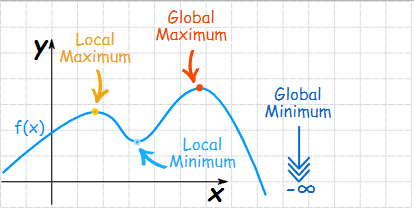
\includegraphics[width=250px]{chapters/03/images/optimums.png}
    \caption{\label{comparatif} \emph{Local and global optimums}, \cite{Optimums0}}
\end{figure}

\paragraph{} Pour des fonctions simples, il est possible d'étudier ces dernières afin trouver un minimum global.
C'est le cas pour des fonctions comme $f(x) = 2 + 1/x$ avec $x \in [1, 3]$ qui à un minimum en 3 où elle vaut $7/3$.
Cependant, dans la réalité, ces fonctions sont beaucoup trop complexes - en taille, en paramètres, en constructions
mathématiques - et nous avons alors recours aux \emph{métaheuristiques} et à la \emph{recherche exhaustive} afin
de trouver des solutions satisfaisantes. Il existe plusieurs métaheuristiques : \emph{algorithmes gloutons, descente
de gradient, recherche tabou, recuit simulé, par essaims particulaires}.. leur implémentation commentée est laissée
en annexe au lecteur curieux, aussi nous attarderons-nous ici sur les domaines d'application.

\paragraph{} Ces algorithmes sont régulièrement utilisés car ils interviennent lorsqu'il n'y a pas de moyen pour 
calculer un optimum de manière mathématique ou lorsque cela prendrait trop de temps. On espère alors obtenir un
résultat \emph{au plus proche} de la réalité. On les retrouve :
\begin{itemize}
    \item En \emph{électronique}, pour améliorer le design de cartes imprimées en minimisant le nombre de fils et 
    en minimisant la place requise par les différents composants.
    \item En \emph{finance}, où elles permettent d'optimiser un porte-feuille d'actions en cherchant à \emph{limiter
    les risques} ou en \emph{maximisant} les gains pour une somme donnée.
    \item En \emph{logistique}, dans des problèmes \emph{d'ordonnancement} comme par exemple créer les horaires pour
    des trains, bus ou avions. On va chercher par exemple à garder le moins possible les véhicules sur place (en gare, 
    aéroport).
    \item En \emph{conception}, pour trouver facilement les formes ou matériaux adéquats, ainsi qu'en \emph{construction}
    pour améliorer les formes des structures porteuses.
    \item Dans le domaine \emph{militaire}, principalement comme aide à l'homme afin \emph{de minimiser l'erreur
    humaine}. 
\end{itemize}

\paragraph{} Les applications des ces métaheuristiques sont donc \emph{diverses et variées}, grâce au caractère \emph{
adaptable} de ces dernières et à leur \emph{faible coût de mise en pratique}. Néanmoins, elle fournissent une
solution \emph{absolue}, et sont donc moins efficaces que d'autres catégories d'algorithmes lorsqu'il s'agit de traiter
de problèmes \emph{particuliers, spécialisés}. La recherche de chemins en est un bon exemple. 

\paragraph{} ------------------------------------

\paragraph{} La recherche de chemins. Théorie des graphes, Bellman-Ford, Dijkstra, A*.
Ouverture sur le GPS et les services type Uber

\paragraph{} ------------------------------------

\paragraph{} La révolution du smartphone. La démocratisation de l'IA dans le smartphone.
Quel avenir pour l'IA ?

\paragraph{} ------------------------------------

\paragraph{Quelles contraintes ?} Quelles sont les conditions techniques nous
permettant d'intégrer de l'IA dans des systèmes ? Y a-t-il des contraintes de
volumétrie, de scalabilité, de puissance de calculs ? Nous verrons comment
l'intégration de systèmes intelligents s'est faire avec plus ou moins de succès
selon et les projets, ainsi que les solutions et évolutions qui ont été apportéées,
permettant de simplifier la mise en place et l'utilisation d'IAs.

\paragraph{} Systèmes simples et systèmes complexes. Des patterns gourmands et
des optimisations parfois compliquées. Parallèle avec le bruteforce. Que donnerait 
une tentative d'application de l'IA (pas du ML !) au calcul du BTC ?

\paragraph{Quels apports et quelle utilité ?} Quels sont les apports \emph{concrets}
de l'IA ? Quels domaines sont les plus concernés ? Est-il possible de distinguer
des \emph{patterns d'implémentation} permettant d'apporter des réponses systématiques
à des problèmes connus ?

\paragraph{Objectif} L'objectif est d'ajouter ici des traitements de données automatisés au section
du Réseau.

